\section{Econometrics}
\textit{This section relies heavily on the theoretical background provided by \cite{wooldridge} and \cite{introR}.}


\subsection{Linear Regression}
Given $n$ distinct \textit{explanatory variables} (also known as \textit{regressors}, \textit{predictors} or \textit{independent variables}), the \textbf{multiple linear regression model} takes the form:

\begin{equation}
    y = \beta_0 + \beta_1 x_1 + \beta_2 x_2 + ... + \beta_n x_n + \epsilon
\end{equation}

where $x_i$ is the i$^{th}$ predictor and $\beta_i$ quantifies the association between that variable and the response. We interpret $\beta_i$ as the \textit{average effect} of a one-unit increase in $x_i$ on $y$, holding all other predictors fixed.

The regression coefficients $\beta_0, \beta_1, ..., \beta_n$ are unknown, and must be estimated from the data. This is usually done through a \textit{least-squares} approach (although other fitting methods exists), where the estimates $\hat{\beta_0}, \hat{\beta_1}, ..., \hat{\beta_n}$ are chosen to minimise the sum of squared residuals:

\begin{equation}
    \sum\limits_{i=1}\limits^n (y_i - x_i ^T b)^2
\end{equation}

Given estimates $\hat{\beta_0}, \hat{\beta_1}, ..., \hat{\beta_n}$, it is then straightforward to predict the response $y$ on the basis of a set of values for the predictors $x_1, x_2, ..., x_n$, using the \textit{fitted value}:

\begin{equation}
    \hat{y} = \hat{\beta_0} + \hat{\beta_1} x_1 + \hat{\beta_2} x_2 + ··· + \hat{\beta_n} x_n
\end{equation}

However, there are three types of uncertainties associated with this prediction:

\begin{enumerate}
    \item The coefficient estimates $\hat{\beta_0}, \hat{\beta_1}, ..., \hat{\beta_n}$ are estimates of the true values $\beta_0, \beta_1, ..., \beta_n$. That is, the least squares plane $\hat{y}$ is only an estimate for the true population regression plane $f(x) = \beta_0 + \beta_1 x_1 + ··· + \beta_n x_n$. The inaccuracy in the coefficient estimates is related to the \textit{reducible error}. We can compute a confidence interval in order to determine how close $\hat{y}$ will be to $y$.

    \item In practice, assuming a linear model for $f(x)$ is almost always an approximation of reality, so there is an additional source of potentially reducible error which we call \textit{model bias}. When we use a linear model, we are in fact estimating the best linear approximation to the true surface. However, here we will ignore this discrepancy, and operate as if the linear model were correct.

    \item Even if we knew $f(x)$ --- that is, even if we knew the true values for $\beta_0, \beta_1, ..., \beta_n$ --- the response value cannot be predicted perfectly because of the random error $\epsilon$.
\end{enumerate}

We use \textit{prediction intervals} to measure how much $\hat{y}$ varies from $y$. Prediction intervals are always wider than confidence intervals, because they incorporate both the error in the estimate for $y$ (the \textit{reducible error}) and the uncertainty as to how much an individual point will differ from the population regression plane (the \textit{irreducible error}).


\subsection{Classifiers: Logit \& Probit Models}
The linear regression model assumes that the response variable $y$ is purely \textit{quantitative}, but in many situations, the response variable is in fact \textit{qualitative} (or \textit{categorical}). For example, eye color takes on values such as blue, brown or green. Predicting a qualitative response for an observation is also sometimes referred as \textit{classifying} that observation, since the observation is assigned to a category.

Two of the most widely-used classifiers are the \textbf{logistic} (or \textit{logit}) and \textbf{probit} regressions. In contrast with the linear model, they are used to regress for the \textit{probability} of a categorical outcome (e.g. $y=0$ or $y=1$).

Recall that for the linear regression model, we have:

\begin{equation}
    y = x'\beta + \epsilon
\end{equation}

Binary outcome models instead estimate the \textit{probability} that $y=1$ as a function of the independent variables:

\begin{equation}
    p = P(y=1 | x) = F(x'\beta)
\end{equation}

Since the probit and logit models are estimated using the maximum likelihood method, an increase in $x$ will increase (decrease) the \textit{likelihood} that $y=1$. In other words, an increase in $x$ makes the outcome of $1$ more or less likely.

The distinction between logit and probit comes from the functional form (or \textit{link function}) of $F$ that each methods uses.

\begin{itemize}
    \item \textbf{Logit}: $F$ is the cdf of the logistic distribution
    $$ F(x'\beta) = \Lambda(x'\beta) = \frac{e^{x'\beta}}{1+e^{x'\beta}} $$

    \item \textbf{Probit}: $F$ is the cdf of the standard normal distribution
    $$ F(x'\beta) = \Phi(x'\beta) = \int_{-\infty}^{+\infty} \phi(z)dz $$
    where $\phi(x) = \frac{1}{\sqrt{2\pi}}\ e^{-\frac{x^2}{2}}$
\end{itemize}

\begin{figure}[!ht]
    \centering
    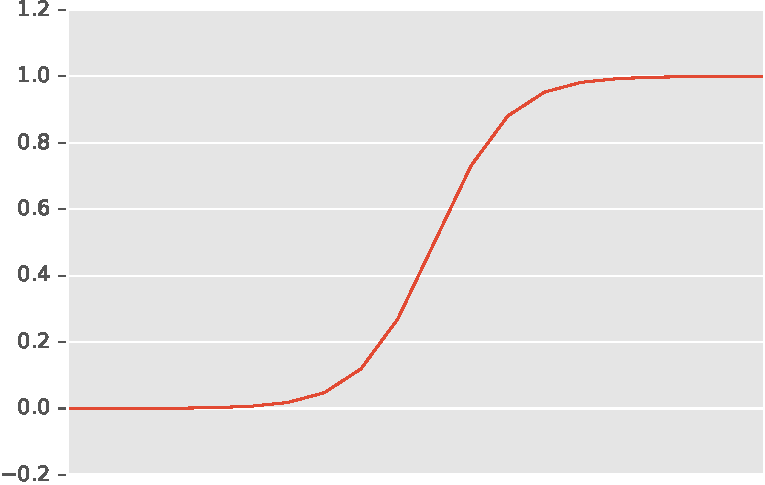
\includegraphics[scale=0.6]{img/logit.pdf}
    \caption{Logit function}
    \label{fig:logit}
\end{figure}

Note that since both link functions are cumulative distribution functions of probability distributions, the predicted values are limited between 0 and 1.

\subsubsection{Marginal effects}
The marginal effect (i.e. the effect of one-unit increase in $x_i$ on $y$, \textit{ceteris paribus}) can be obtained by simply taking the partial derivative of $y$ with respect to the variable of interest $x_i$:

\begin{equation}
    EM(x_j) = \frac{\partial y}{\partial x_j}
\end{equation}

With the linear model, we trivially obtain $\beta_1$ as the marginal effect of $x_1$, that is, the marginal effects are simply the coefficients and they do not depend on $x$.

For the logit and probit models, the marginal effects are slighly more complicated because of the non-linearity introduced by the link function:

\begin{equation}
    EM(x_j) = \frac{\partial \mathbf{E}[y|x]}{\partial x_j} = \beta_j F'(x'\beta)
\end{equation}

The marginal effects thus depend on $x = (x_1, ..., x_n)$, so we need to estimate them at a specific value of $x$, which is typically chosen to be the mean value ––- in other words, the vector of characteristics of the "average observation".

Thus, for the logit model, we have that:
$$
    EM(x_j) = \beta_j\Lambda(x'\beta)(1-\Lambda(x'\beta)) = \beta_j\frac{e^{x'\beta}}{(1+e^{x'\beta})^2}
$$

and for the probit model:
$$
    EM(x_j) = \beta_j\Phi'(x'\beta) = \beta_j\phi(x'\beta) = \beta_j
$$
where $\phi(x) = \frac{1}{\sqrt{2\pi}}\ e^{-\frac{x^2}{2}}$.

\subsubsection{Interpretation}

\begin{itemize}
    \item An increase in $x$ increases (decreases) the probability that $y=1$ by the marginal effect
expressed as a percentage
    \begin{itemize}
        \item For dummy independent variables, the marginal effect is expressed in comparison to the
    base category ($x=0$).
        \item For continuous independent variables, the marginal effect is expressed for a one-unit
    change in $x$.
    \end{itemize}
    \item We interpret both the sign and the magnitude of the marginal effects.
    \item The probit and logit models produce almost identical marginal effects (up to a constant).
\end{itemize}

\subsubsection{Coefficients}
A nice property of the linear regression model is that \textit{the marginal effects are the coefficients}, which means that we can evaluate the marginal effect of each regressor $x_i$ simply by looking at the summary output from the regression.

This does not hold for logit and probit models, because of the presence of the link function, as discussed in the previous section. However, we can devise a simple "rule-of-thumb" to approximate the marginal effect from the coefficients. Recall that for logit and probit models:

\begin{equation}
    EM(x_j) = \frac{\partial \mathbf{E}[y|x]}{\partial x_j} = \beta_j F'(x'\beta)
\end{equation}

Now, using maximum value of the $F'$ function, we obtain an upper-bound approximation for the marginal effect directly from the coefficients in the summary table:

\begin{equation}
    EM(x_j) \approx \beta_j \max F'(x'\beta)
\end{equation}

For the logit model, $\max \Lambda'(x) = \Lambda'(0) = \frac{1}{4}$ and for the probit model, $\max \phi(x) = \phi(0) = \frac{1}{\sqrt{2\pi}} = \frac{1}{2.5}$ --- thus, our simple "rule-of-thumb" for finding marginal effects can be summarised as follows:

\begin{itemize}
    \item \textbf{Logit}: $EM(x_j) \approx \beta_j/4$
    \item \textbf{Probit}: $EM(x_j) \approx \beta_j/2.5$
\end{itemize}

% TODO: odds ratios
% \subsubsection{Odds ratios/relative risk for the logit model}
% The odds ratio or relative risk is $\frac{p}{1-p}$ and measures the probability that $y=1$ relative
% to the probability that $y=0$.

% $$p = \frac{e^{x'\beta}}{1+e^{x'\beta}}$$
% $$\frac{p}{1-p} = e^{x'\beta}$$
% $$\ln \frac{p}{1-p} = x'\beta$$

% An odds ratio of $2$ means that the outcome $y=1$ is twice as likely as the outcome of $y=0$. Odds
% ratios are estimated with the logistic model.
